\begin{frame}
	\frametitle{Gleichgewichtszustände in komplexen Systemen}
	\only<1|handout:1>{
	\begin{figure}
		\centering
		
\includegraphics[trim={0cm 0cm 0cm 1.15cm}, clip, width=0.35\linewidth]{bilder/kipppunkte/pendulum}
		
\includegraphics[width=0.5\linewidth]{bilder/kipppunkte/stones}
	\end{figure}
	}
	\only<2|handout:0>{
	\begin{figure}
		\centering
		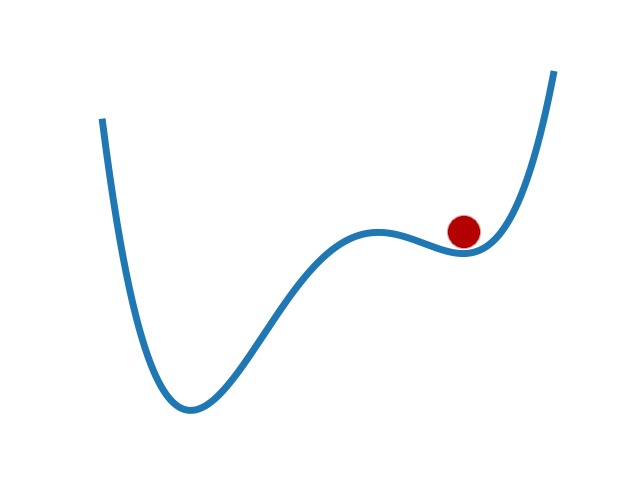
\includegraphics[width=0.7\linewidth]{bilder/kipppunkte/potential1}
	\end{figure}
	}
	\only<3|handout:2>{
	\begin{figure}
		\centering
		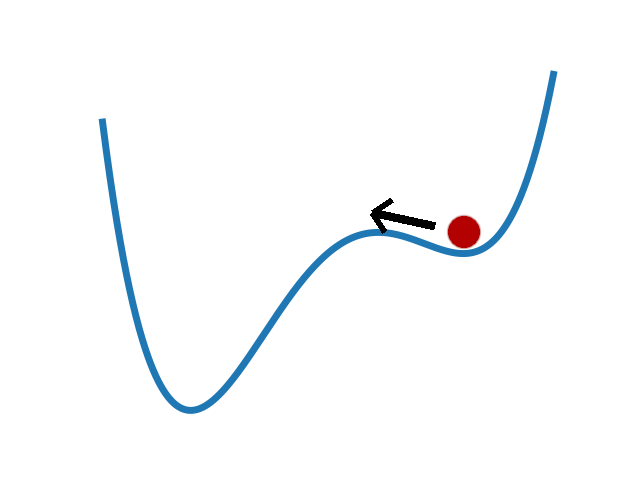
\includegraphics[width=0.7\linewidth]{bilder/kipppunkte/potential2}
	\end{figure}
	}
	\only<4|handout:0>{
	\begin{figure}
		\centering
		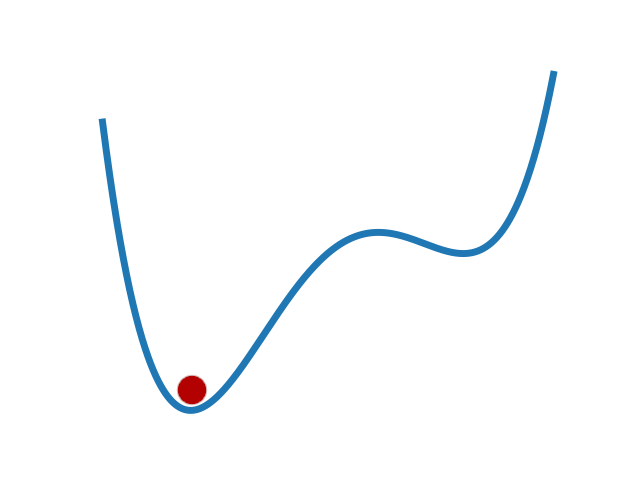
\includegraphics[width=0.7\linewidth]{bilder/kipppunkte/potential3}
	\end{figure}
	}
	\note{
		\begin{itemize}
			\item<1->[] Dynamische Systeme können sich in verschiedenen Gleichgewichtszuständen befinden
			\item<1->[] Das Klima an sich ist ein dynamisches System, aber auch die einzelnen Komponenten für sich
			\item<1->[] Einfachste Form des Gleichgewichts (absolut) stabiles Gleichgewicht, Beispiel Pendel
			\begin{itemize}
				\item<1-> Wenn man nicht dauerhaft von außen Energie zuführt, ist es immer im selben Zustand
			\end{itemize}
			\item<1->[] Gleichgewichte können auch labil sein, Beispiel Steinhaufen
			\begin{itemize}
				\item<1-> Aktuell ist das System zwar in einem Gleichgewichtszustand, aber die kleinste Änderung führt sofort zu einer Änderung
			\end{itemize}
			\item<2->[] Komplexe Systeme können auch mehrere Gleichgewichtszustände haben
			\begin{itemize}
				\item<2-> labil, stabil und semi-stabil können alle vorhanden sein
			\end{itemize}
			\item<2->[] Das System ist dann gegenüber kleinen Änderungen unempfindlcih
			\item<2->[] Wenn die Änderung aber groß genug ist, tritt ein dauerhafter neuer Zustand ein
		\end{itemize}
	}
\end{frame}

\begin{frame}
	\frametitle{Beispiele für Kipppunkte des Klimasystems}
	\begin{columns}
		\column[t]{0.5\linewidth}
		\begin{figure}
			\centering
			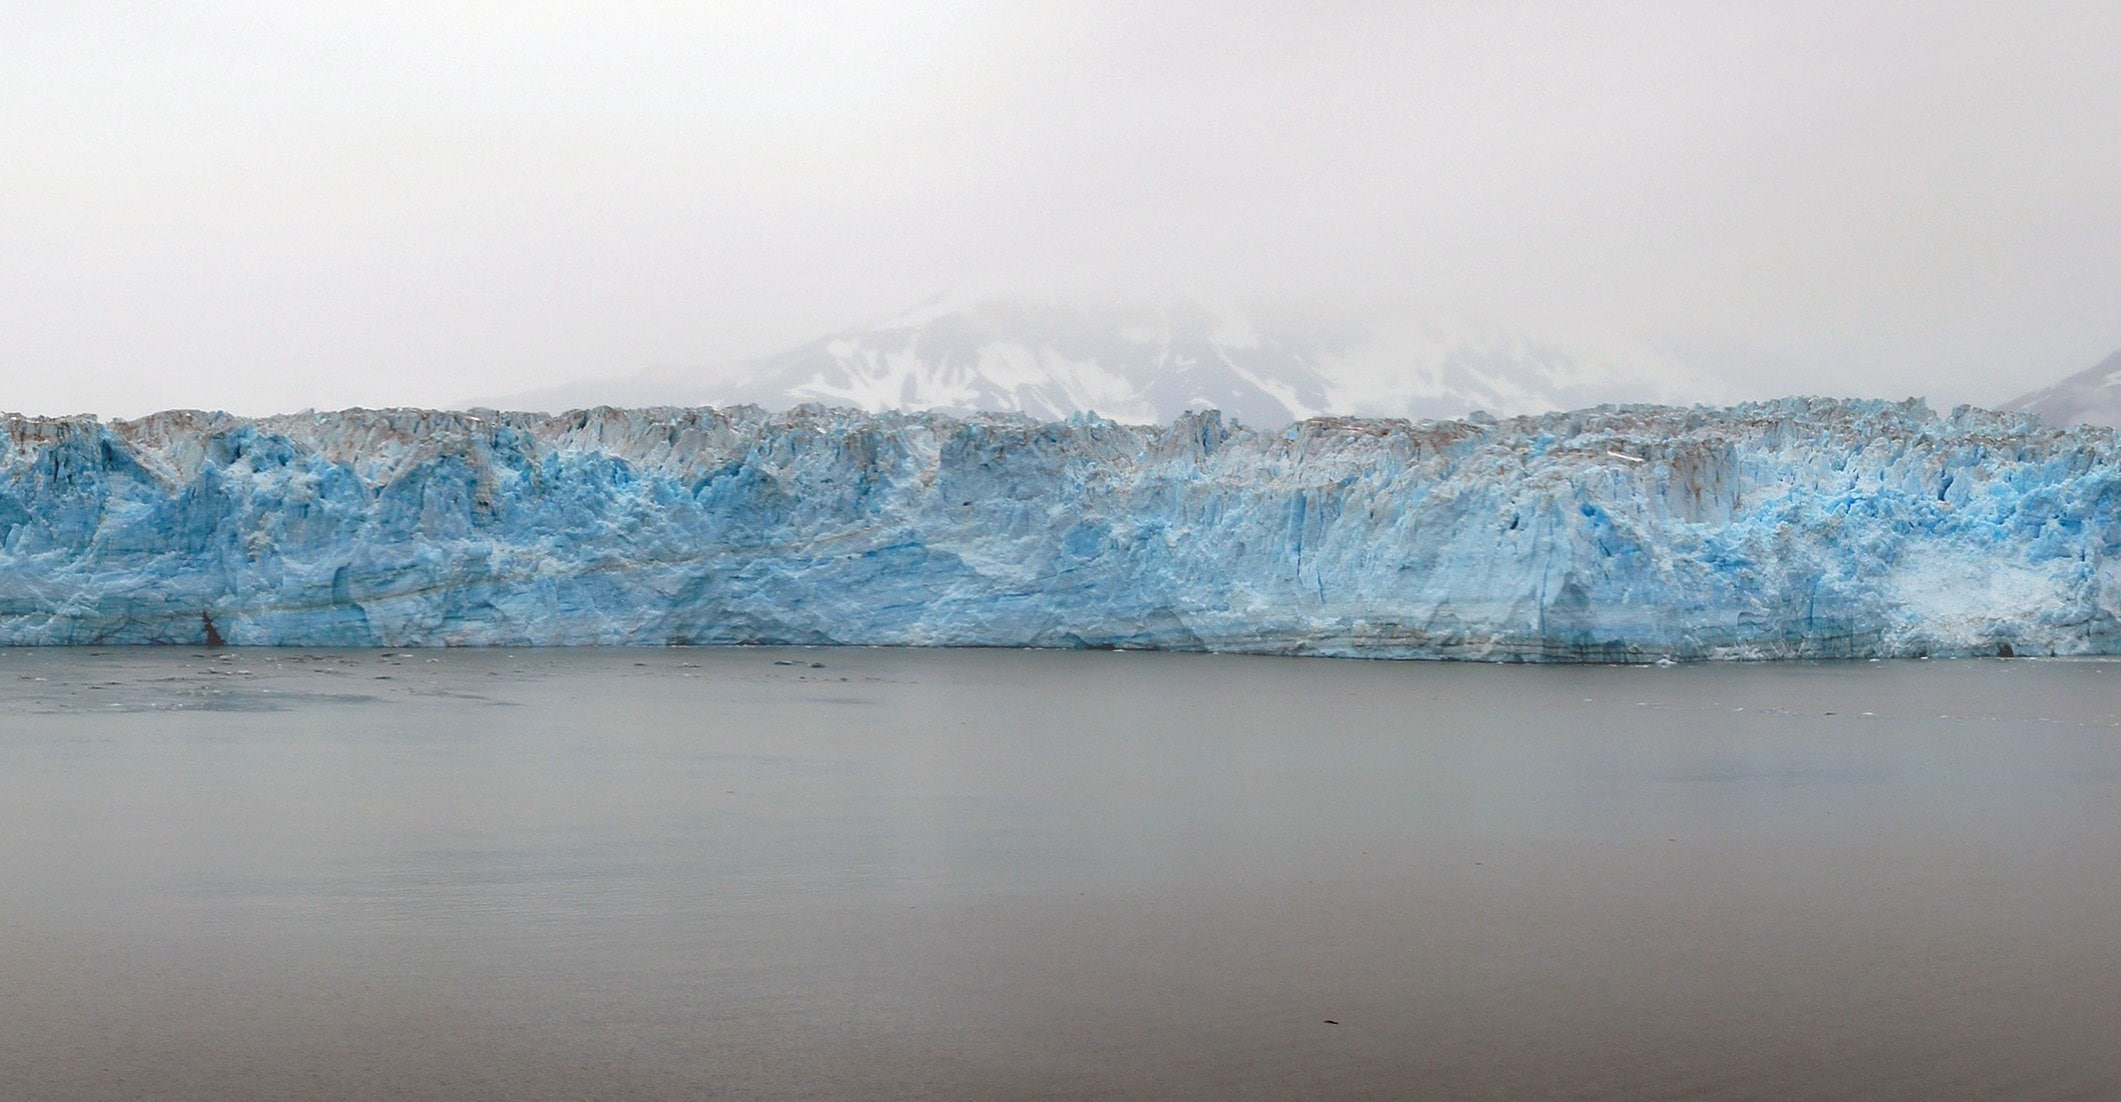
\includegraphics[trim={11cm 2.7cm 0cm 2cm}, clip, width=0.9\linewidth]{bilder/groenland}
			\caption{Eisschild auf Grönland}
		\end{figure}
		\begin{itemize}
			\item Wenn der Kilometer dicke Eispanzer auf Grönland schmilzt, könnte der Meeresspiegel um bis zu 7 Meter steigen
		\end{itemize}
		\column[t]{0.5\linewidth}
		\begin{figure}
			\centering
			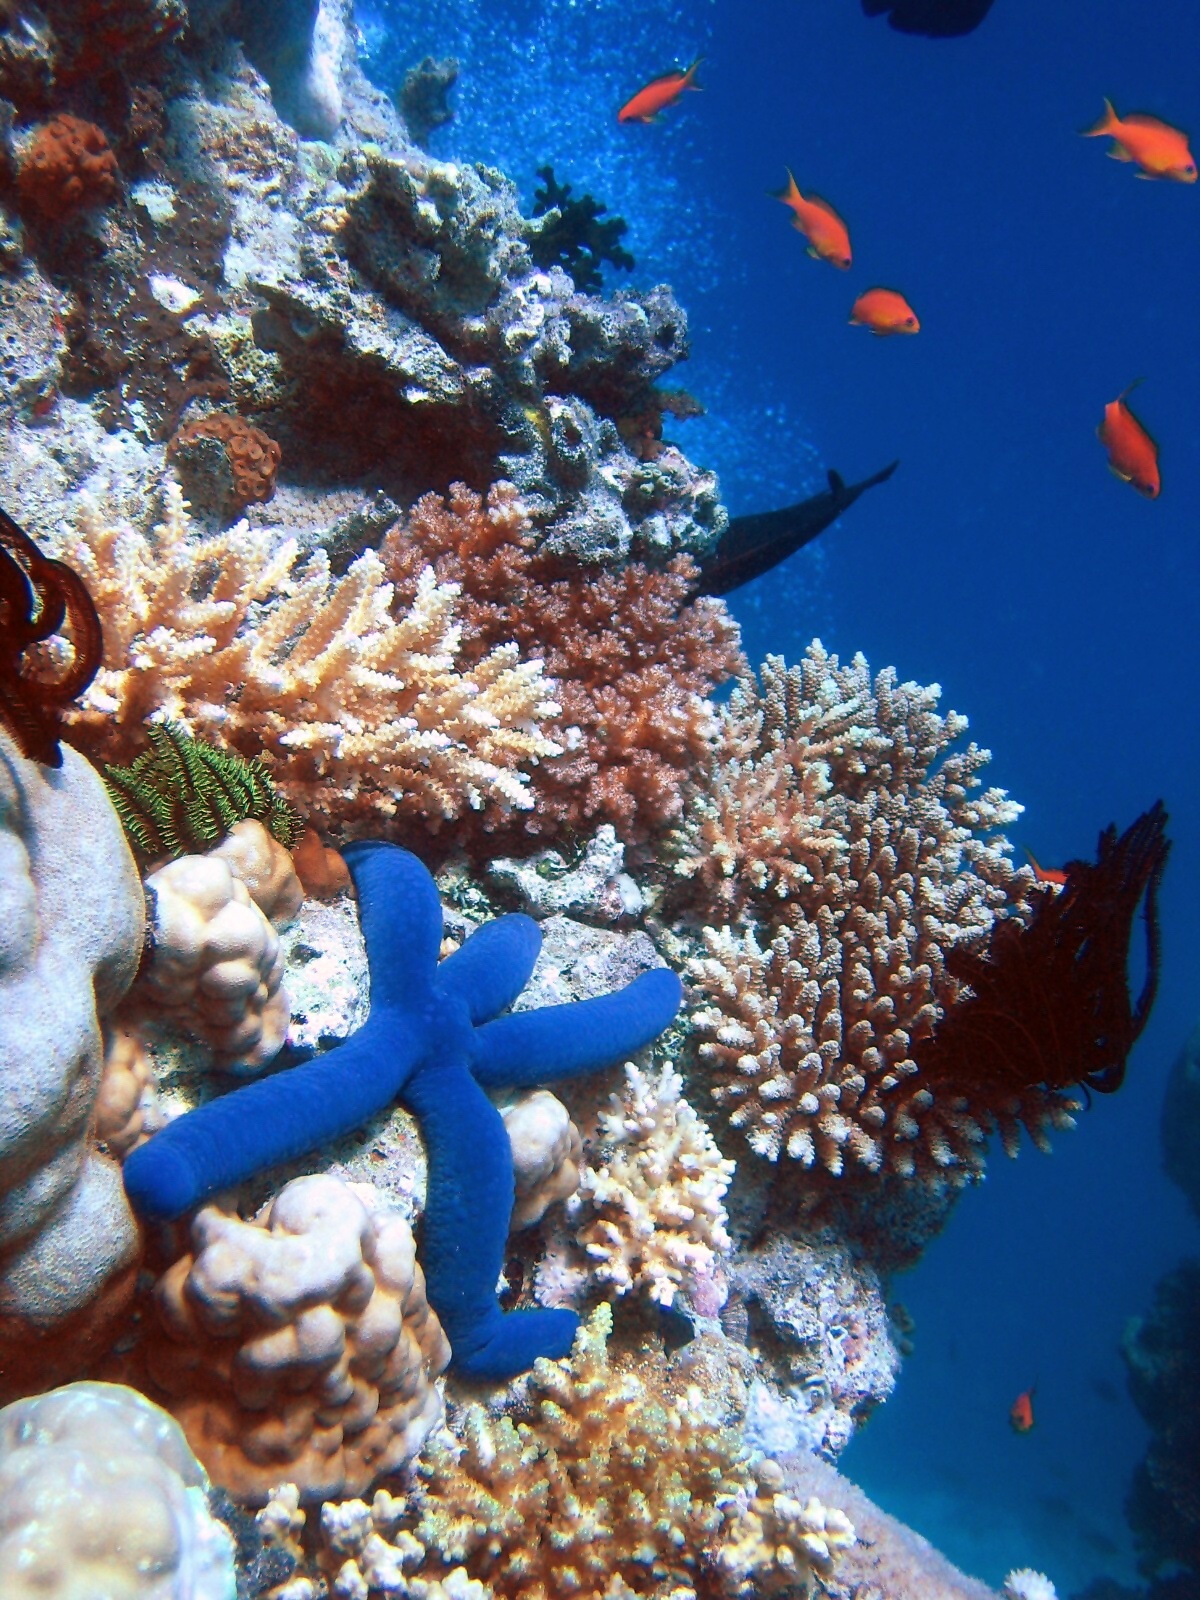
\includegraphics[height=0.9\linewidth, angle=90]{bilder/great_barrier_reef}
			\caption{Korallen vor Australien}
		\end{figure}
		\begin{itemize}
			\item Die weltweiten Korallenriffe leiden unter Versauerung der Ozeane und erhöhter Temperatur
		\end{itemize}
	\end{columns}

	\note{
		\begin{itemize}
			\item[] Grönland ist auf einer Fläche von \SI{1.8e6}{\kilo\meter\squared} (etwa 5 mal Deutschland) mit einem bis zum \SI{3}{\kilo\meter} dicken Eispanzer bedeckt.
			\item[] Der Eispanzer unterliegt durch Schmelzen im Sommer und Schneefall im Winter einer ständigen Veränderung.
			\item[] Außerdem geht an den Küsten kontinuierlich Eis verloren.
			\item[] Bei höheren Temperaturen wird das Wechselspiel aus Schmelzen und Wachstum gestört, außerdem gleitet das Eis auf Schmelzwasser schneller ins Meer
			\item[] In Folge kann es zu einem raschen abschmelzen kommen und dadurch bedingt zu einem Anstieg des Meeresspiegels um bis zu \SI{7}{\meter} über Jahrhunderte
			\item[] Dieser Kipppunkt könnte bereits erreicht sein [King]. Auch eine sofortiger Stopp der globalen Temperaturerhöhung würde das abschmelzen dann nicht mehr verhindern.
			\item[] Das Eis in der Westantartikis verhält sich ähnlich, könnte jedoch etwas stabiler sein. Das Eis in der Ostantarktis scheint bisher weniger gefährdet.
			\item[] Durch Erhöhung des CO$_2$ Gehaltes wird das Meerwasser langsam sauer. Das wirkt sich negativ auf viele Lebewesen aus, insbesondere Korallen, da ihnen in sauerer Umgebung nicht genug Kalk zur Verfügung steht.
			\item[] Die höheren Temperaturen führen außerdem vermehrt zur Korallenbleiche. Bei dieser sterben die Algen auf der Oberfläche der Korallen ab, was die Koralle selbst ebenfalls schädigt.
			\item[] Ab einem gewissen Grad der Schädigung werden die Korallenriffe zunehmend absterben, selbst wenn sich CO$_2$ Gehalt und Temperatur nicht weiter erhöhen, da der Hitzestress dauerhaft zu hoch ist.
		\end{itemize}
	}
\end{frame}

\begin{frame}
	\frametitle{Kipppunkte des Klimasystems}
	\only<1|handout:1>
	{
	\begin{figure}
		\centering
		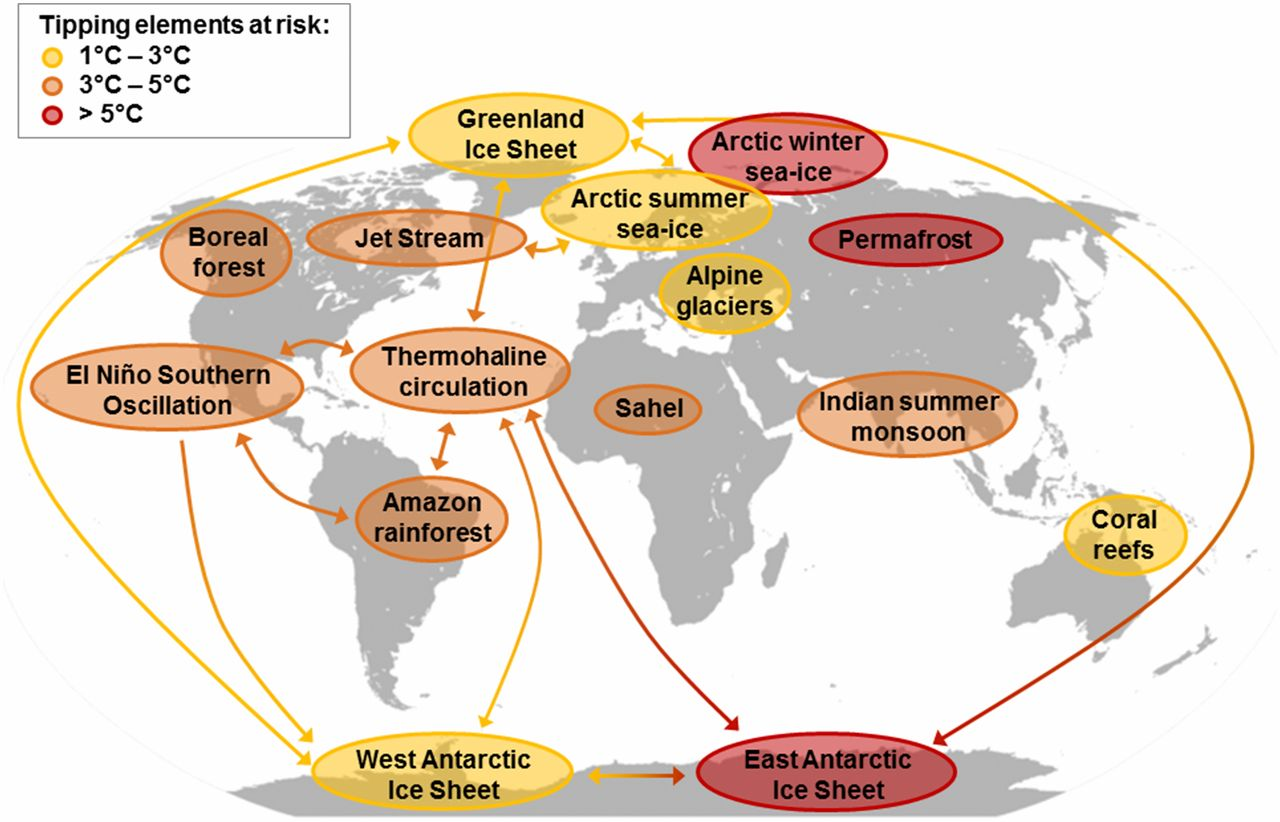
\includegraphics[width=0.825\linewidth]{bilder/kipppunkte/tipping_elements}
		\caption{Die wichtigsten bekannten möglichen Kipppunkte mit ihren Wechselwirkungen, Quelle: Lenton}
		\label{fig:tippingelements}
	\end{figure}
	}
	\only<2|handout:2>
	{
	\begin{figure}
		\centering
		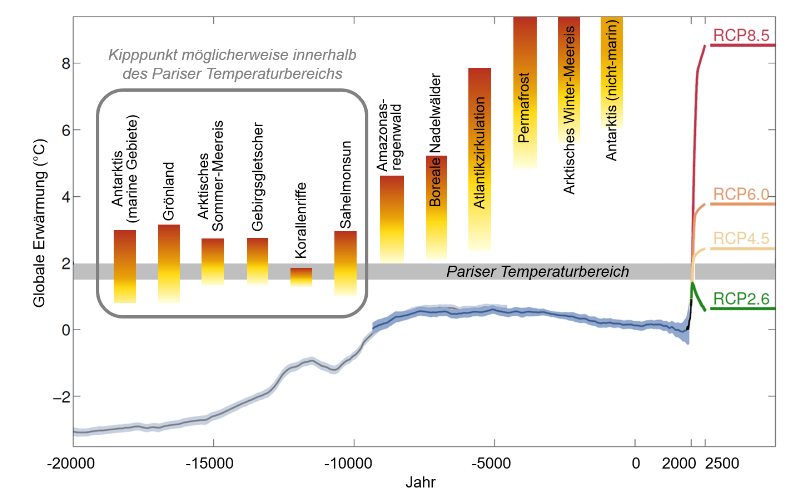
\includegraphics[width=0.85\linewidth]{bilder/kipppunkte/bereiche}
		\caption{Erwärmungsbereiche in denen ein auslösen bestimmter Kippelemente wahrscheinlich ist, Quelle: Rahmstorf}
		\label{fig:tippingelements2}
	\end{figure}
	}

	\note<1->{
	\vspace{-2em}
	\begin{itemize}
		\item[] Die 15 wichtigsten bekannten Kipppunkte und ihre Wechselwirkungen.
		\item[] Für kleine Änderungen ist der Zusammenhang zwischen anstieg der Treibhausgaskonzentration und anstieg der Temperatur nahezu proportional
		\item[] Es gibt aber auch Effekte, die sich auf Wetter und Klima auswirken, welche sich aber einer gewissen Temperatur selbst verstärken $\rightarrow$ Eis-Albedo-Rückkoplung
		\item[] Auch die thermohaline Zirkulation der Wassermassen ist ein Beispiel dafür, da diese ja gerade durch die Wassertemperatur angetrieben wird. Änderungen der Zirkulation können dann zu lokalen Änderungen des Klimas führen
		\item[] Selbstverstärkende Effekte haben die Eigenschaft ab einem gewissen Punkt kaum noch aufhaltbar zu sein, man spricht daher von \textit{Kipppunkten} im Klimasystem.
	\end{itemize}
	}
	\note<2>{
	\begin{itemize}
		\item[] Sowohl die Zeitskala auf der so ein Effekt abläuft (siehe Trägheit), als auch die Temperatur ab der dieser einsetzen kann, ist für jeden Kippunkt unterschiedlich
		$\rightarrow$ Wann ein Kipppunkt erreicht ist, ist relativ unsicher, was passiert wenn er erreicht ist, relativ sicher
		\item[UBA] \textit{Das Klimasystem ist kein träges und gutmütiges Faultier, sondern es kann sehr abrupt und heftig reagieren}
		\item[] I.A. sind diese Kipppunkte deutlich schwerer zu modelieren, da ihre Folgen beim eintreten massiv sind, und sie sich in einer Art Kettenreaktion auch gegenseitig auslösen können (Pfeile in Abbildung).
		\item[] Wenn viele dieser Kippelemente erreicht werden, könnte die Erde insgesamt in ein neues, wärmes klimatisches Gleichgewicht geraten ("Hothouse Earth"). Es könnte daher unmöglich sein, das Klima bei einer beliebigen Temperatur zu "parken".
		\item[RCP] Representative Concentration Pathway, Zahl ist der Strahlungsantrieb (radiative forcing) im Jahr 2100 (Strahlungsantrieb: Änderung der Energiebilanz der Erde)
		\item[1990] \SI{417}{ppm} (RF: 2,165)
		\item[2018] \SI{496}{ppm} (RF: 3,101)
	\end{itemize}
}
\end{frame}
